%% 
%% Created in 2018 by Martin Slapak
%% last update:		2020-02-09
%%
%% Based on file for NRP report LaTeX class by Vit Zyka (2008)
%% enhanced for MI-MVI (2018) and tuned for BI-PYT (2020)
%%
%% Compilation:
%% >pdflatex report
%% >bibtex report
%% >pdflatex report
%% >pdflatex report

\documentclass[czech]{pyt-report}

\usepackage[utf8]{inputenc} 
\usepackage{placeins}

\title{PAC-MAN}

\author{Matěj Frnka}
\affiliation{ČVUT--FIT}
\email{frnkamat@fit.cvut.cz}

\def\file#1{{\tt#1}}

\begin{document}

\maketitle

Replika japonské počítačové hry PAC-MAN.

%%%%%%%%%%%%%%%%%%%%%%%%%%%%%%%%%%%%%%%%%%%%%%%%%%%%%%%%%%%%%%%%%%%%%%%%%%%%%%%%
\section{Úvod}


Pac-man je 2d arkádová hra vytvořena roku 1980 japonským vývojářem Namco. Hra nemá konec, hráč se pouze snaží přežít co nejdéle a získat při tom co nejvyšší skóre. To se dá získat tím, že pac-man sebere žluté \textit{jídlo}.\par
Není to ovšem tak jednoduché. Během hry se pac-mana snaží chytit \textit{duchové}, kteří pac-mana po většinu hry pronásledují. Když ho chytí, pac-man ztratí život. Dohromady má životy tři, pokud o všechny přijde, hra končí.\par
Pac-man není proti \textit{duchům} úplně bezbranný. Na mapě se nacházejí \textit{super-jídla}, díky kterým pac-man získá schopnost \textit{jíst duchy} – za prvního pak dostane 200 bodů, za dalšího 400, poté 600 a za posledního 800 bodů.
\section{Cíl}
Cílem této semestrální práce je naprogramovat hru pac-man. Kód hry musí být lehce upravitelný. Programátor by měl být schopen rychle zkoušet různé možnosti chování \textit{duchů} a rychle měnit mapu, aby mohl experimentovat s různými způsoby hry. Ovládání hráčů by mělo být lehce upravitelné, aby se semestrální práce dala použít jako základ pro vývoj umělé inteligence pac-mana pomocí strojového učení.


%%%%%%%%%%%%%%%%%%%%%%%%%%%%%%%%%%%%%%%%%%%%%%%%%%%%%%%%%%%%%%%%%%%%%%%%%%%%%%%%
\section{Pravidla pohybu}
Pac-man se pohybuje ve čtyřech směrech – nahoru, dolů, doleva, doprava. V jakýkoliv čas smí zatočit jakýmkoliv z těchto směrů, pokud mu v cestě nebrání zeď. Pokud hráč zadá směr blokovaný zdí, pac-man si vstup zapamatuje a změní směr, jakmile to půjde. Pokud pac-man narazí na stěnu, zastaví se.\par
\begin{figure}[h]
  \centering\leavevmode
  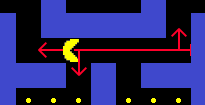
\includegraphics[width=.45\linewidth]{img/pac-man_directions.png}\vskip-0.5cm
  \caption{Možné směry z daného bodu}
  \label{fig:par-y}
\end{figure}
\textit{Duchové} mají pravidla pro pohyb podobná jako pac-man. Nemohou se ale otočit o 180$^{\circ}$  stupňů a nikdy se nezastaví. Pokud hráč zná chování \textit{duchů}, může toho využít a úmyslně je poslat špatným směrem.


%%%%%%%%%%%%%%%%%%%%%%%%%%%%%%%%%%%%%%%%%%%%%%%%%%%%%%%%%%%%%%%%%%%%%%%%%%%%%%%%
\section{Umělá inteligence}
\textit{Duchové} mají čtyři módy chování.
\subsection{Mód \textit{rozptýlení}}
V módu \textit{rozptýlení} se \textit{duchové} snaží dostat do určitého bodu, každý \textit{duch} má svůj bod, v nynější konfiguraci je každý v jednom rohu mapy.\par Tento mód se používá pro rozptýlení \textit{duchů} po mapě. Je aktivován pod dobu sedmi sekund na začátku hry.
\subsection{Mód \textit{lovec}}
Mód \textit{lovec} je defaultní mód chování, je aktivován pokud zrovna neprobíhá žádný jiný.\par
\textit{Duch} se vždy snaží dostat do určitého bodu. Pozice tohoto bodu je u každého \textit{ducha} určena jinak. Kdyby byl tento bod u každého \textit{ducha} stejný, \textit{duchové} by se v průběhu hry mohli potkat a kvůli stejnému rozhodování, už by se nikdy nerozdělili. Proto má každý \textit{duch} vlastní algoritmus určování cílového bodu.
\subsubsection{\textit{Duch Blinky}}
\textit{Blinky} má ze všech \textit{duchů} nejjednodušší chování. Pronásleduje pac-mana – jeho cílový bod je stejný jako pac-manova pozice

\begin{figure}[h]
  \centering\leavevmode
  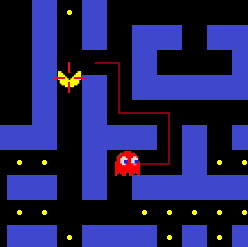
\includegraphics[width=.5\linewidth]{img/blinky_ai.png}
  \caption{Ukázka chování \textit{blinky}}
  \label{fig:par-y}
\end{figure}
\FloatBarrier
\subsubsection{\textit{Duch Pinky}}
\textit{Pinky} je komplikovanější. Snaží se pac-manovi naběhnout do cesty. Proto je jeho cílový vždy bod o dva bloky před pac-manem

\begin{figure}[h]
  \centering\leavevmode
  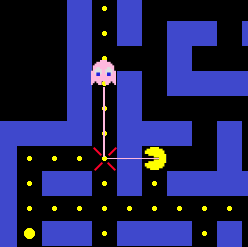
\includegraphics[width=.5\linewidth]{img/pinky_ai.png}
  \caption{Ukázka chování \textit{pinky}}
  \label{fig:par-y}
\end{figure}
\FloatBarrier
\subsubsection{\textit{Duch Inky}}
\textit{Inkyho} cílový bod závisí na pozici \textit{ducha Blinky}. Pokud by se nakreslila čára procházející \textit{Blinkyho} pozicí a bodem o jeden blok vzdáleným před pac-manem. \textit{Inkyho} cílový bod byl na takové čáře přímo naproti pozici Blinkyho.

\begin{figure}[h]
  \centering\leavevmode
  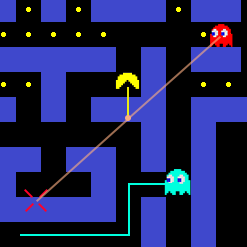
\includegraphics[width=.5\linewidth]{img/inky_ai.png}
  \caption{Ukázka chování \textit{inky}}
  \label{fig:par-y}
\end{figure}
\FloatBarrier
\subsubsection{\textit{Duch Clyde}}
\textit{Clyde} pronásleduje pac-mana stejně jako \textit{Blinky}. Pokud se ale přiblíží do okruhu 4 bloků, lekne se a přepne se do módu \textit{rozptýlení}. Jakmile z okruhu vyjde, přepne se zpět do módu lovec.

\begin{figure}[h]
  \centering\leavevmode
  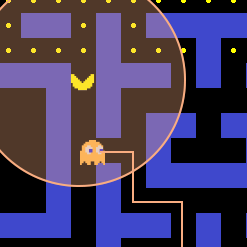
\includegraphics[width=.5\linewidth]{img/clyde_ai.png}\vskip-0.5cm
  \caption{Ukázka chování \textit{clyde}}
  \label{fig:par-y}
\end{figure}
\FloatBarrier
\subsection{Mód \textit{Vystrašení}}
Tento mód nastane potom, co hráč sní \textit{super-jídlo}.\par
\textit{Duchové} změní svou animaci, zpomalí se a směr vybírají náhodně. V tomto módu je pac-man může \textit{jíst}, pokud tak nastane, \textit{duch} změní svůj mód na mrtvý.\par
Celý mód trvá 5 sekund. Poslední 1.5 sekundy \textit{duchové} začnou blikat, aby indikovali, že se brzy změní buď do stavu rozptýlení nebo lovení.
\subsection{Mód \textit{Mrtvý}}
\textit{Duch} změní animaci a zrychlí. Podobně jako v módu rozptýlení se \textit{duch} snaží dostat do určitého bodu. Tento bod se nachází v počáteční místnosti \textit{duchů}. Jakmile se \textit{duch} dostane do tohoto bodu, změní svůj mód mód podle času kola buď na rozptýlení nebo na lovení.
\subsection{Hledání cesty k bodům}
Většina výše uvedených módů vybere bod, kam se \textit{duch} snaží dostat. Při vybírání cesty \textit{duch} nemusí vždy vybrat tu nejrychlejší. Toto je záměrně dodává hře \textit{chaotický} dojem. Při hledání cesty \textit{duch} porovná možné směry. Vybere si vždy směr, který je blíže k cílovému bodu, tím se pak vydá.
\begin{figure}[h]
  \centering\leavevmode
  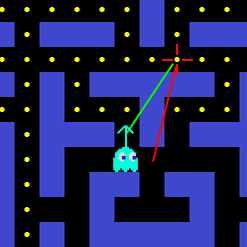
\includegraphics[width=.5\linewidth]{img/ai.png}
  \caption{Hledání cesty}
  \label{fig:par-y}
\end{figure}
%%%%%%%%%%%%%%%%%%%%%%%%%%%%%%%%%%%%%%%%%%%%%%%%%%%%%%%%%%%%%%%%%%%%%%%%%%%%%%%%
% --- VYSLEDKY
\onecolumn
\section{Výsledky}

Byl splněn hlavní účel projektu. Pomocí pouze pythonu 3.7.4, pygletu a numpy jsem vytvořil hru pac-man. Díky způsobu, kterým je hra naprogramována, je velmi lehké ji upravit. Například pro přidání nebo odebrání \textit{duchů} stačí upravit pár řádků v jediné funkci, přidání dalších pac-manů je podobné. Mapa lze změnit pomocí změny jediné proměnné. Pro změnu chování \textit{duchů} stačí implementovat třídu dědící z třídy TargetBehaviour a dát ji při vytváření do konstrukturu \textit{ducha}, ten se pak bude chovat podle ní, podobně lze u více \textit{duchů} používat stejné chování a zkoušet, jaký to má efekt na hratelnost.
%%%%%%%%%%%%%%%%%%%%%%%%%%%%%%%%%%%%%%%%%%%%%%%%%%%%%%%%%%%%%%%%%%%%%%%%%%%%%%%%
% --- ZAVER
\section{Závěr}
Díky lehké upravitelnosti může hra sloužit jako základ pro mnohem rozsáhlejší projekty jako je procedurální generování map jakýchkoliv velikostí, trénování pac-mana a\textit{duchů} pomocí strojového učení nebo může jako prototyp k rozsáhlejší hře inspirované pac-manem.\par
Semestrální práce mě zaujala a jakmile budu mít více času, začnu experimentovat se strojovým učením pac-mana. Vzhledem k tomu, že se \textit{duchové} chovají až na mód vystrašení deterministicky, bude zajímavé sledovat jaké strategie pac-man využije proti jejich chování.

\begin{figure}[h]
  \centering\leavevmode
  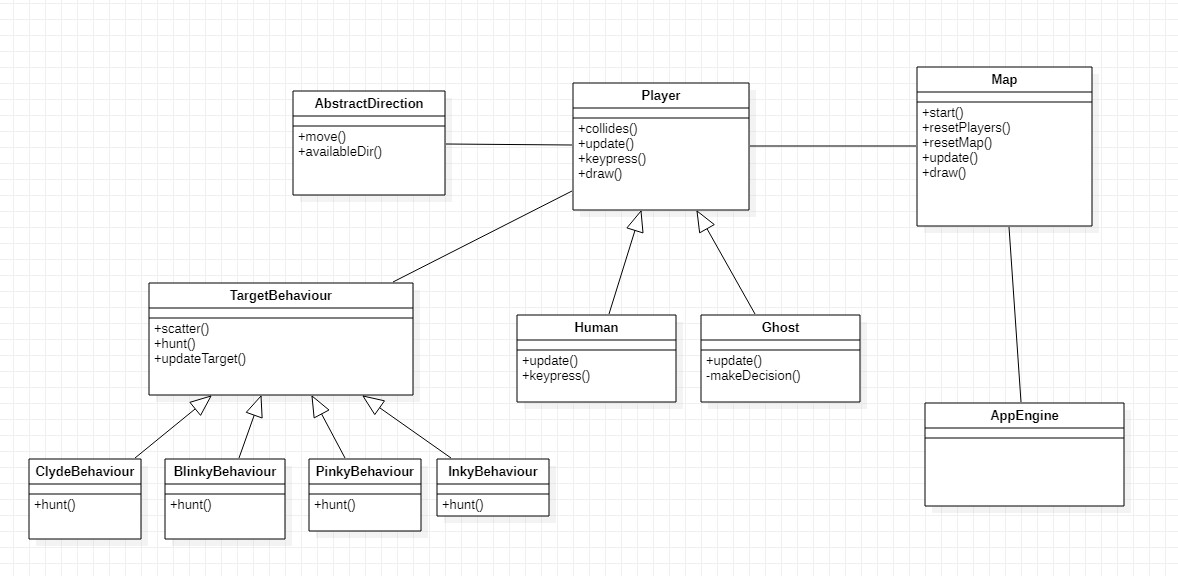
\includegraphics[width=1\linewidth]{img/class_diagram.jpg}
  \caption{Rozložení tříd v programu}
  \label{fig:par-y}
\end{figure}


%%%%%%%%%%%%%%%%%%%%%%%%%%%%%%%%%%%%%%%%%%%%%%%%%%%%%%%%%%%%%%%%%%%%%%%%%%%%%%%%
% --- Bibliography
\nocite{Pittman}
\nocite{ghosts}
%\bibliographystyle{plain-cz-online}
\bibliography{reference}


\end{document}
